\documentclass[border=6pt]{standalone}
\usepackage{amsmath,amssymb}
\usepackage{tikz}
\usetikzlibrary{arrows.meta,calc,decorations.pathreplacing,patterns,shapes.geometric,positioning,shadings,plotmarks}

\begin{document}
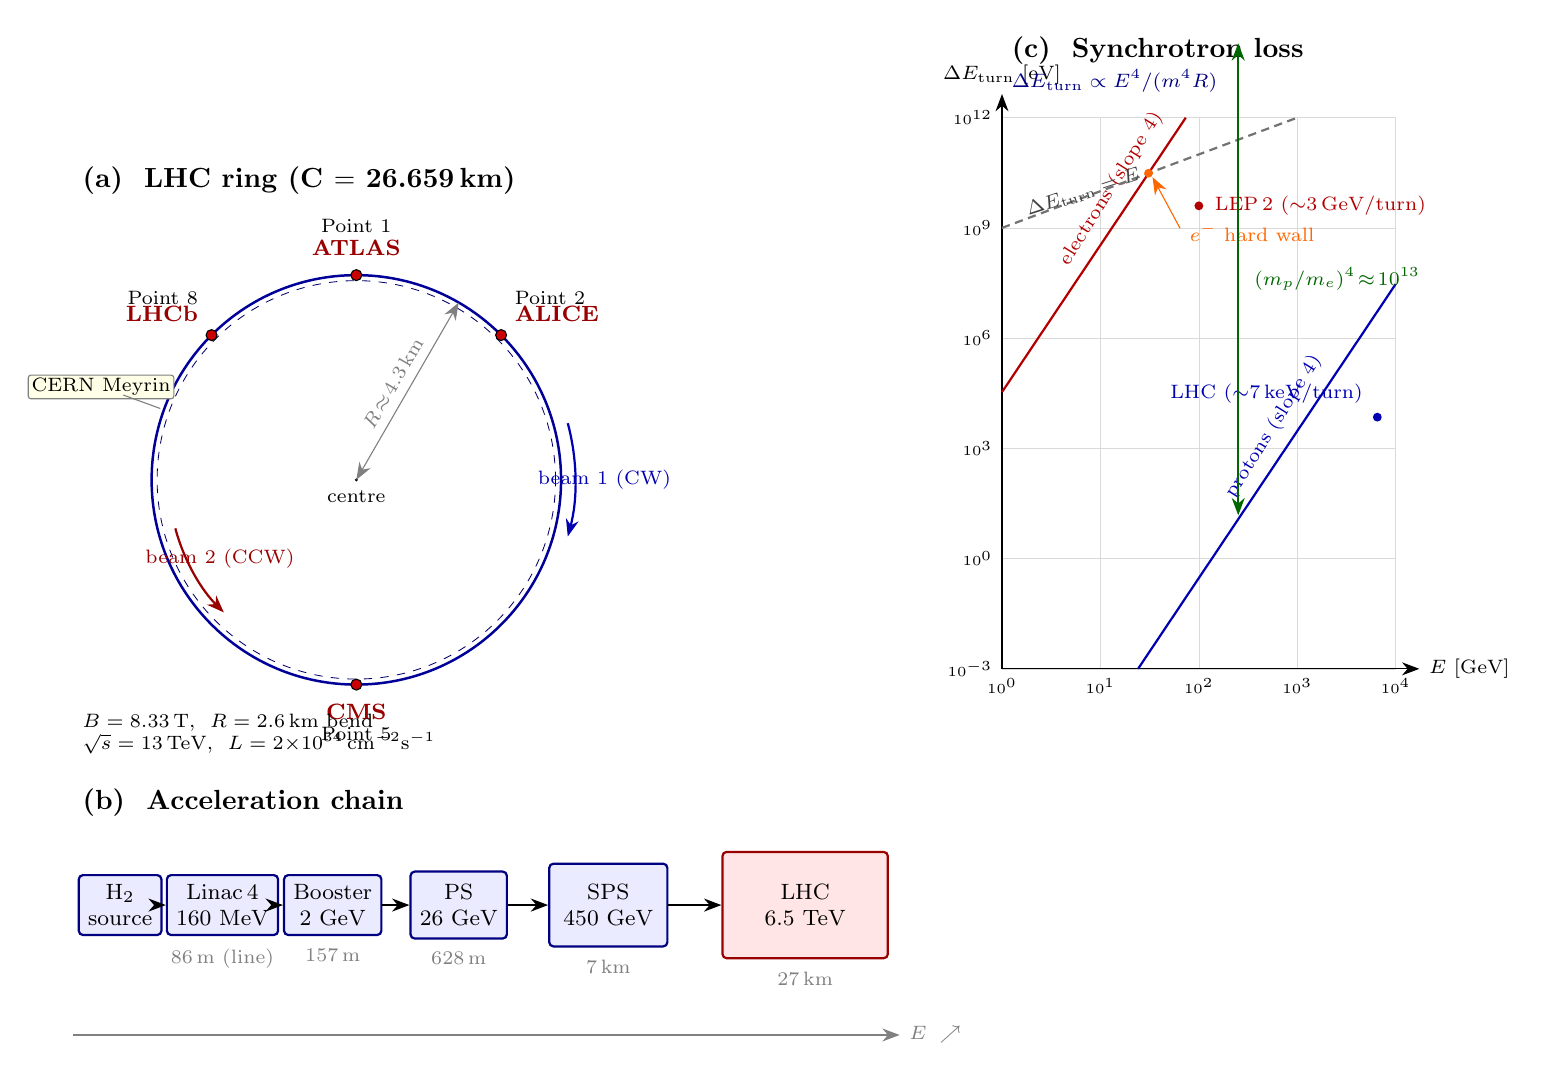
\begin{tikzpicture}[
    >={Stealth[length=2.2mm]},
    font=\small,
    node distance=0pt,
    expt/.style={circle,draw=black,fill=red!80!black,inner sep=1.4pt},
    chainbox/.style={draw=blue!50!black,fill=blue!8,thick,rounded corners=1.5pt,align=center,font=\footnotesize}
]

%% =====================================================================
%% TOP-LEFT : LHC 27 km RING WITH FOUR DETECTORS
%% =====================================================================
\begin{scope}[shift={(0,0)}]
  % Outer reference grid
  \node[anchor=south west,font=\bfseries] at (-3.6,3.5) {(a)\ \ LHC ring (C $=$ 26.659\,km)};

  % Ring (geometric centre radius approx 4.3 km, drawn as 2.6 cm)
  \def\Rring{2.6}
  \draw[blue!60!black,line width=0.9pt] (0,0) circle (\Rring);
  % Subtle inner second line for the two-beam pipe
  \draw[blue!40!black,line width=0.3pt,dashed] (0,0) circle (\Rring-0.07);

  % Geocentre marker
  \fill[black] (0,0) circle (0.6pt);
  \node[font=\scriptsize,below=0.5pt] at (0,0) {centre};

  % Compass: Point 1 (ATLAS) at North
  % LHC convention: P1 (ATLAS) N, P2 (ALICE) NE, P5 (CMS) S, P8 (LHCb) NW
  % Angles measured from East, counter-clockwise (TikZ default)
  \def\angATLAS{90}
  \def\angALICE{45}
  \def\angCMS{270}
  \def\angLHCb{135}

  \foreach \ang/\name/\det/\anch in {
      \angATLAS/Point 1/ATLAS/below,
      \angALICE/Point 2/ALICE/below left,
      \angCMS/Point 5/CMS/above,
      \angLHCb/Point 8/LHCb/below right}{
    \node[expt] (\det) at (\ang:\Rring) {};
  }
  \node[anchor=south,font=\footnotesize\bfseries,red!60!black] at ($(ATLAS)+(0,0.12)$) {ATLAS};
  \node[anchor=south,font=\scriptsize] at ($(ATLAS)+(0,0.42)$) {Point 1};

  \node[anchor=south west,font=\footnotesize\bfseries,red!60!black] at ($(ALICE)+(0.05,0.05)$) {ALICE};
  \node[anchor=south west,font=\scriptsize] at ($(ALICE)+(0.05,0.27)$) {Point 2};

  \node[anchor=north,font=\footnotesize\bfseries,red!60!black] at ($(CMS)+(0,-0.12)$) {CMS};
  \node[anchor=north,font=\scriptsize] at ($(CMS)+(0,-0.42)$) {Point 5};

  \node[anchor=south east,font=\footnotesize\bfseries,red!60!black] at ($(LHCb)+(-0.05,0.05)$) {LHCb};
  \node[anchor=south east,font=\scriptsize] at ($(LHCb)+(-0.05,0.27)$) {Point 8};

  % Two counter-rotating beam arrows (small arcs on the ring)
  \draw[->,thick,blue!70!black]
      ([shift={(15:\Rring+0.18)}]0,0) arc (15:-15:\Rring+0.18);
  \node[font=\scriptsize,blue!70!black] at (0:\Rring+0.55) {beam 1 (CW)};
  \draw[->,thick,red!60!black]
      ([shift={(195:\Rring-0.22)}]0,0) arc (195:225:\Rring-0.22);
  \node[font=\scriptsize,red!60!black] at (210:\Rring-0.6) {beam 2 (CCW)};

  % Radius annotation
  \draw[<->,gray] (0,0) -- (\angATLAS-30:\Rring) node[midway,above,font=\scriptsize,sloped] {$R\!\approx\!4.3$\,km};

  % CERN Meyrin reference (off-ring, NW exterior)
  \node[draw=black!50,fill=yellow!10,rounded corners=1pt,font=\scriptsize,inner sep=1.2pt]
       at (160:\Rring+0.85) {CERN Meyrin};
  \draw[gray,thin] (160:\Rring+0.55) -- (160:\Rring+0.05);

  % Spec labels
  \node[font=\scriptsize,align=left,anchor=north west]
       at (-3.6,-2.85) {$B=8.33$\,T,\ \ $R=2.6$\,km bend\\$\sqrt{s}=13$\,TeV,\ \ $L=2{\times}10^{34}$\,cm$^{-2}$s$^{-1}$};
\end{scope}

%% =====================================================================
%% BOTTOM : ACCELERATION CHAIN
%% =====================================================================
\begin{scope}[shift={(0,-5.4)}]
  \node[anchor=south west,font=\bfseries] at (-3.6,1.0) {(b)\ \ Acceleration chain};

  % Source
  \node[chainbox,minimum width=0.9cm,minimum height=0.55cm] (src)
       at (-3.0,0) {H$_2$\\source};

  % Five-stage chain. Box width grows with circumference of the machine.
  % Linac 4 (linear, ~86 m) -> Booster (~157 m) -> PS (628 m)
  % -> SPS (~7 km) -> LHC (27 km).  We use sqrt scaling on the area so
  % the LHC box is visibly biggest yet still fits.
  \node[chainbox,minimum width=0.7cm,minimum height=0.55cm] (linac)
       at (-1.7,0) {Linac\,4\\160 MeV};
  \node[chainbox,minimum width=0.85cm,minimum height=0.7cm] (booster)
       at (-0.3,0) {Booster\\2 GeV};
  \node[chainbox,minimum width=1.1cm,minimum height=0.85cm] (ps)
       at (1.3,0) {PS\\26 GeV};
  \node[chainbox,minimum width=1.5cm,minimum height=1.05cm] (sps)
       at (3.2,0) {SPS\\450 GeV};
  \node[chainbox,minimum width=2.1cm,minimum height=1.35cm,fill=red!10,draw=red!60!black] (lhc)
       at (5.7,0) {LHC\\6.5 TeV};

  \draw[->,thick] (src) -- (linac);
  \draw[->,thick] (linac) -- (booster);
  \draw[->,thick] (booster) -- (ps);
  \draw[->,thick] (ps) -- (sps);
  \draw[->,thick] (sps) -- (lhc);

  % Approximate circumference labels
  \node[font=\scriptsize,gray,below=1pt] at (linac.south)   {86\,m (line)};
  \node[font=\scriptsize,gray,below=1pt] at (booster.south) {157\,m};
  \node[font=\scriptsize,gray,below=1pt] at (ps.south)      {628\,m};
  \node[font=\scriptsize,gray,below=1pt] at (sps.south)     {7\,km};
  \node[font=\scriptsize,gray,below=1pt] at (lhc.south)     {27\,km};

  % Energy axis arrow under the chain
  \draw[->,gray] (-3.6,-1.65) -- (6.9,-1.65) node[right,font=\scriptsize] {$E\;\nearrow$};
\end{scope}

%% =====================================================================
%% RIGHT : LOG-LOG  Delta E_turn  vs  E   (electron vs proton)
%% =====================================================================
\begin{scope}[shift={(8.2,-2.4)}]
  % Axis frame.  x: log10(E/GeV) in 0..4 -> width 5 cm.  y: log10(DeltaE/eV)
  % range -3..12 -> height 7 cm.   So 1 dec x = 1.25 cm, 1 dec y = 0.4667 cm.
  \def\xa{0} \def\xb{4}
  \def\ya{-3} \def\yb{12}
  \pgfmathsetmacro{\Wx}{5.0}    % cm per (xb-xa)
  \pgfmathsetmacro{\Hy}{7.0}    % cm per (yb-ya)
  \pgfmathsetmacro{\sx}{\Wx/(\xb-\xa)}
  \pgfmathsetmacro{\sy}{\Hy/(\yb-\ya)}

  % Helper: convert (logE, logDE) to cartesian
  % point = ((\logE-\xa)*\sx, (\logDE-\ya)*\sy)

  % Grid
  \foreach \ix in {0,1,2,3,4}{
      \pgfmathsetmacro{\px}{(\ix-\xa)*\sx}
      \draw[gray!30,very thin] (\px,0) -- (\px,\Hy);
      \node[font=\tiny,below] at (\px,0) {$10^{\ix}$};
  }
  \foreach \iy in {-3,0,3,6,9,12}{
      \pgfmathsetmacro{\py}{(\iy-\ya)*\sy}
      \draw[gray!30,very thin] (0,\py) -- (\Wx,\py);
      \node[font=\tiny,left] at (0,\py) {$10^{\iy}$};
  }
  % Frame
  \draw[->] (0,0) -- (\Wx+0.3,0) node[right,font=\scriptsize] {$E$ [GeV]};
  \draw[->] (0,0) -- (0,\Hy+0.3) node[above,font=\scriptsize] {$\Delta E_{\mathrm{turn}}$ [eV]};

  % Title and formula
  \node[font=\bfseries,anchor=south west] at (0,\Hy+0.55) {(c)\ \ Synchrotron loss};
  \node[font=\scriptsize,anchor=south west,blue!50!black]
       at (0,\Hy+0.20) {$\Delta E_{\mathrm{turn}}\propto E^4/(m^4 R)$};

  %% --- Electron line: log10(DE_e[eV]) = log10(88.5e6) + 4 logE - log10 R[m]
  %% with R = 2600 m  ->  log10(88.5e6/2600) = log10(34038) = 4.532
  %% so y_e = 4.532 + 4*x   (x = log10 E[GeV])
  %% At x=0:  y=4.53.    At x=4:  y=20.53 (off-chart).
  %% On-chart: clamp to y<=12 -> intersection at 4x = 12 - 4.532 -> x = 1.867
  \pgfmathsetmacro{\eA}{4.532}                 % intercept
  \pgfmathsetmacro{\xeMax}{(12-\eA)/4}          % where electron line hits y=12
  \pgfmathsetmacro{\peAx}{(\xa-\xa)*\sx}
  \pgfmathsetmacro{\peAy}{(\eA-\ya)*\sy}
  \pgfmathsetmacro{\peBx}{(\xeMax-\xa)*\sx}
  \pgfmathsetmacro{\peBy}{(12-\ya)*\sy}
  \draw[red!70!black,thick] (\peAx,\peAy) -- (\peBx,\peBy);
  \node[red!70!black,font=\scriptsize,anchor=south west,rotate=58]
       at ($(\peAx,\peAy)!0.4!(\peBx,\peBy)$) {electrons (slope $4$)};

  %% LEP 2 marker: E = 100 GeV (logE=2), Delta E ~ 4 GeV = 4e9 eV (log = 9.6)
  \pgfmathsetmacro{\xLEP}{(2-\xa)*\sx}
  \pgfmathsetmacro{\yLEP}{(9.6-\ya)*\sy}
  \fill[red!70!black] (\xLEP,\yLEP) circle (1.6pt);
  \node[font=\scriptsize,red!70!black,anchor=west] at (\xLEP+0.08,\yLEP)
       {LEP\,2 ($\sim$3\,GeV/turn)};

  %% --- Proton line: shift down by log10[(m_p/m_e)^4] = 4*log10(1836) = 13.06
  \pgfmathsetmacro{\pA}{\eA-13.06}              % = -8.53
  %% On-chart range: y must be >= -3   ->  -8.53 + 4 x >= -3 -> x >= 1.383
  \pgfmathsetmacro{\xpMin}{(-3-\pA)/4}
  \pgfmathsetmacro{\ppAx}{(\xpMin-\xa)*\sx}
  \pgfmathsetmacro{\ppAy}{(-3-\ya)*\sy}
  \pgfmathsetmacro{\ppBx}{(\xb-\xa)*\sx}
  \pgfmathsetmacro{\ppBy}{(\pA+4*\xb-\ya)*\sy}  % at x=4: pA + 16 = 7.47
  \draw[blue!70!black,thick] (\ppAx,\ppAy) -- (\ppBx,\ppBy);
  \node[blue!70!black,font=\scriptsize,anchor=south west,rotate=58]
       at ($(\ppAx,\ppAy)!0.4!(\ppBx,\ppBy)$) {protons (slope $4$)};

  %% LHC marker: E = 6500 GeV (logE = 3.813), Delta E ~ 7 keV = 7e3 eV (log=3.85)
  \pgfmathsetmacro{\xLHC}{(3.813-\xa)*\sx}
  \pgfmathsetmacro{\yLHC}{(3.85-\ya)*\sy}
  \fill[blue!70!black] (\xLHC,\yLHC) circle (1.6pt);
  \node[font=\scriptsize,blue!70!black,anchor=south east] at (\xLHC-0.06,\yLHC+0.05)
       {LHC ($\sim$7\,keV/turn)};

  %% --- Hard-wall horizontal: Delta E = E (eV).  E[GeV]=10^x -> E[eV]=10^{x+9}
  %% the line y = x+9.  Intersection with electron line:  x+9 = 4.532+4x -> x=1.489
  %% (i.e. ~31 GeV).  Intersection with proton line: x+9 = -8.53+4x -> x = 5.84 (off-chart).
  %% Draw the line y = x + 9 across the panel:
  \pgfmathsetmacro{\hAx}{(\xa-\xa)*\sx}
  \pgfmathsetmacro{\hAy}{(\xa+9-\ya)*\sy}      % at x=0: y=9
  \pgfmathsetmacro{\hBx}{(\xb-\xa)*\sx}
  \pgfmathsetmacro{\hBy}{(\xb+9-\ya)*\sy}      % at x=4: y=13 (clamp)
  %% Clamp upper end to y=12: at y=12, x=3.
  \pgfmathsetmacro{\hBxC}{(3-\xa)*\sx}
  \pgfmathsetmacro{\hByC}{(12-\ya)*\sy}
  \draw[densely dashed,gray!90!black,thick] (\hAx,\hAy) -- (\hBxC,\hByC);
  \node[gray!50!black,font=\scriptsize,anchor=west,rotate=18]
       at (\hAx+0.2,\hAy+0.18) {$\Delta E_{\mathrm{turn}}=E$};

  %% Mark the electron hard-wall crossing (~31 GeV)
  \pgfmathsetmacro{\xHW}{(1.489-\xa)*\sx}
  \pgfmathsetmacro{\yHW}{(10.489-\ya)*\sy}
  \fill[orange!80!red] (\xHW,\yHW) circle (1.6pt);
  \draw[orange!80!red,->,thin] (\xHW+0.4,\yHW-0.7) -- (\xHW+0.05,\yHW-0.05);
  \node[font=\scriptsize,orange!80!red,anchor=west]
       at (\xHW+0.4,\yHW-0.75) {$e^-$ hard wall};

  %% Gap arrow: 13 decades between curves at x=2
  \pgfmathsetmacro{\gxA}{(2.4-\xa)*\sx}
  \pgfmathsetmacro{\gyHigh}{(\eA+4*2.4-\ya)*\sy}
  \pgfmathsetmacro{\gyLow}{(\pA+4*2.4-\ya)*\sy}
  \draw[<->,thick,green!40!black] (\gxA,\gyHigh-0.05) -- (\gxA,\gyLow+0.05);
  \node[font=\scriptsize,green!40!black,anchor=west]
       at (\gxA+0.08,{0.5*(\gyHigh+\gyLow)}) {$(m_p/m_e)^4\!\approx\!10^{13}$};

\end{scope}

\end{tikzpicture}
\end{document}
